



\begin{figure*}[tb]
\centering
\includegraphics[width=0.78\textwidth]{illustrations/refactoringTree.eps}
\vspace{-6pt}
\caption{Equivalence classes with various representations. DBB = Double-Bounded, SNG = Single Bounded, LWB = Lower Bounded, CCC = Custom Character Class and LIT = Literal. We use concrete regexes in the representations for illustration. However, the A's in the LWB group (or B's in DBB group, S's in SNG group, and so forth) abstractly represent any pattern that could be operated on by a repetition modifier (e.g., literal characters, character classes, or groups). The same is true for the literals used in all the representations. }
\vspace{-6pt}
\label{fig:refactoringTree}
\end{figure*}


\section{Research Questions}
\label{sec:study}
%After defining the equivalence classes and potential  regex refactorings as described in Section~\ref{sec:refactoring}, we wanted to know which representations in the equivalence classes  are considered desirable and which might be smelly. Desirability for regexes can be defined many ways, including maintainable,  understandable, and performance. 
%%As prior work has shown that regexes are difficult to read~\cite{}, 
%We focus on refactoring for understandability.

To explore regex comprehension and identify smells, we answer the following research questions: \\
%We define regex understandability two ways. First,  we  present people with regexes exemplifying some of the more common characteristics and ask them comprehension questions along two directions: determine which of a list of strings are matched by the regex, and compose a string that is matched by the regex. Second, assuming that common programming practices are more understandable than uncommon practices, we explore the frequencies of each representation from Figure~\ref{fig:refactoringTree} using thousands of regexes scraped from Python projects. 

\noindent {\textbf{RQ1:}} {\em Which regex representations are most understandable?}
To answer RQ1, we conduct a study in which programmers are presented with a regex and asked comprehension questions about its matching behavior.  By comparing accuracy between regexes that match the same language but are expressed differently (e.g., \verb!tri[a-f]3! and \verb!tri(a|b|c|d|e|f)3!), we can measure understandability and identify code smells. This analysis requires identification of equivalence classes for regexes. By inspecting  nearly 14,000 regexes extracted from Python projects in a publicly available dataset~\cite{chapman2016}, we formed an initial set of five equivalence classes to explore. \\
% as measured by identifying matching strings and by composing matching strings

\noindent {\textbf{RQ2:}} {\em Which regex representations have the strongest {community support} based on  frequency?} % each representation appears in regexes in open source Python projects?}
To answer RQ2, we explore the publicly available regex dataset~\cite{chapman2016} and use the presence and absence of language features as a proxy for community support, where more frequently-used features are assumed to be more understandable.\\

\noindent {\textbf{RQ3:}}  {\em Which regex representations are most desirable (i.e., least smelly) based on both community support and understandability?}
Based on RQ1 and RQ2, we identify smelly and non-smelly regex features  based on a combination of comprehension metrics and community support. \\

Next, we present the equivalence classes, analysis and results for each RQ, and a unified discussion.







%\footnote{same dataset used in prior work~\cite{chapman2016}}
\section{Equivalence Classes}
\label{sec:refactoring}
%After studying over 13,000 distinct regex strings from Python projects, 
To explore understandability, we defined an initial set of equivalence classes for regexes. 
Using the publicly available behavioral clusters of Python regexes~\cite{chapman2016}, we manually identified several representations that appeared in many of the larger clusters. 
While not a complete set of equivalence classes, this is the first work to explore regex  understandability, and these equivalence classes provide an initial testbed for exploration.
% (Section~\ref{sec:futureequivclasses} identifies other equivalence classes left to explore in future work.)

%For example,  \verb!AAA*! and \verb!AA+! are semantically identical, except one uses the star operator (indicating zero or more repetitions) and the other uses the plus operator (indicating one or more repetitions).
%Both match strings with two or more \verb!A!'s.
Figure~\ref{fig:refactoringTree} shows five equivalence classes in grey boxes and semantically equivalent \emph{representations} in white boxes with identifiers in white circles. For example, LWB is an equivalence class with representations L1, L2, and L3. Regexes \verb!AAA*! and \verb!AA+!  map to L2 and L3, respectively.
%, along with the L1 representation, \verb!A{2,}!.
%The undirected edges between the representations define possible refactorings.
%Identifying the best direction for each arrow in the possible refactorings is discussed in Section~\ref{sec:rq3}.
%We use concrete regexes in the representations to more clearly illustrate examples of the representations. However, the \verb!A!'s in the LWB group abstractly represent any pattern that could be operated on by a repetition modifier (e.g., literal characters, character classes, or groups). The same is true for the literals used in all the representations. 
Next, we describe each equivalence class group. 

\subsection{Custom Character Class Group}
The Custom Character Class (CCC) group has regex representations that use the custom character class language feature or can be represented by such a feature.
%The character class regex language feature is a fundamental feature found in all language flavors since GREP (check this?).
 A custom character class matches a set of alternative characters.  For example, the regex \verb!c[ao]t! will match strings ``cat" and ``cot" because, between the \verb!c! and \verb!t!, there is a custom character class, \verb![ao]!, that specifies either \verb!a! or \verb!o! (but not both) must be selected.  We use the term \emph{custom} to differentiate these classes  from the default character classes, : \verb!\d!, \verb!\D!, \verb!\w!, \verb!\W!, \verb!\s!, \verb!\S! and \verb!.!,  provided by most regex libraries, though the default classes can be encapsulated in a custom character class. %, as is the case with the C4 representation.
 % For the purposes of our analysis, a negated custom character class (like \verb![^abc]!) is handled separately.
%Next, we provide descriptions of each representation in this equivalence class:
\begin{description}  \itemsep -1pt
\item[C1:] Any pattern that contains a (non-negative) custom character class with  a range feature like \verb![a-f]! as shorthand for all of the characters between `a' and `f' (inclusive) belongs to  C1.


\item[C2:] Any pattern that contains a (non-negative) custom character class  without any shorthand representations, specifically ranges or defaults (e.g., \verb![012]! is in C2, but \verb![0-2]! is not).


\item[C3:] Any pattern with a character class expressed using negation, indicated by a caret (i.e., \verb!^!) followed by a custom character class.
% (including literal characters, default character classes and ranges).  
For example, the pattern \verb![^ao]! matches every character \emph{except} \verb!a! or \verb!o!. 
% If the applicable character set is known (e.g., ASCII, UTF-8, etc.), then any non-negative character class can be represented as a negative character class.  For example, assuming an ASCII charset that has 128 characters: \verb!\x00-\x7f!, a character class representing the lower half: \verb![\x00-\x3f]! can be represented by negating the upper half: \verb![^\x40-\x7f]!.


\item[C4:]Any pattern using a default character class such as \verb!\d! or \verb!\W! within a (non-negative) character class. % belongs to the C4 node.  

\item[C5:]  These can be transformed into custom character classes by removing the ORs and adding square brackets (e.g., \verb!(\d|a)! in C5 is equivalent to \verb![\da]! in C4). All custom character classes expressed as an OR of length-one sequences, including defaults or other custom classes, are in C5\footnote{An OR cannot be directly negated, it there is no edge between C3 and C5}. 
\end{description}

Note that a pattern can belong to multiple representations. For example,  \verb![a-f\d]! belongs to both C1 and C4.  
%The edge between C1 and C4 represents the opportunity to express the same pattern as \verb![a-f0-9]! by transforming the default digit character class into a range.  This transformed version would only belong to the C1 node.
%\todoNow{add a thing}

\subsection{Double-Bounded Group}
The Double-Bounded (DBB) group contains all regex patterns that use some repetition defined by a (non-equal) lower and upper boundary.  For example,  \verb!pB{1,3}s! represents a \verb!p! followed by one to three sequential \verb!B! patterns, then followed by a single \verb!s!.  This matches ``pBs", ``pBBs", and ``pBBBs".

\begin{description}  \itemsep -1pt
\item[D1:] Any pattern that  uses the curly brace repetition with a lower and upper bound, such as  \verb!pB{1,3}s!. 
%Note that  \verb!pB{1,3}s! can become \verb!pBB{0,2}s! by pulling the lower bound out of the curly braces and into the explicit sequence (or visa versa). Nonetheless, it would still be part of D1.
%, though this within-node refactoring on D1 is not discussed in this work.
\item[D2:] Any pattern that uses the questionable (i.e., \verb!?!) modifier implies a lower-bound of zero and an upper-bound of one (and hence is double-bounded). 
%For example, when a double-bounded regex has zero on the lower bound, such as \verb!pBB{0,2}s!  in D1, an equivalent representation in D2 contains questionable modifiers,  creating \verb!pBB?B?s!.
\item[D3:] Any pattern that has a repetition with a lower and upper bound and is expressed using ORs (e.g.,  \verb!pB{1,3}s! becomes \verb!pBs|pBBs|pBBs! by expanding on each option in the boundaries).
%Note also that a pattern can belong to multiple nodes in the DBB group, for example, \verb!(a|aa)X?Y{2,4}! belongs to all three nodes.
% =======
% \item[D1:] Any pattern that  uses the curly brace repetition with a lower and upper bound where the upper and lower bounds are different, such as  \verb!pB{1,3}s!, belongs to the D1 node.
% Note that  \verb!pB{1,3}s! can become \verb!pBB{0,2}s! by pulling the lower bound out of the curly braces and into the explicit sequence (or visa versa). Nonetheless, it would still be part of D1, though this within-node refactoring on D1 is not discussed in this work.
% \item[D2:] Any pattern that uses the questionable (i.e., \verb!?!) modifier implies a lower-bound of zero and an upper-bound of one, and belongs to D2. For example, when a double-bounded regex has zero on the lower bound, as is the case with \verb!pBB{0,2}s!  in D1, transforming it to D2 involves replacing the curly braces with $n$ questionable modifiers, where $n$ is the upper bound,  creating \verb!pBB?B?s!.
% \item[D3:] Any pattern that has a repetition with a lower and upper boundary and is expressed using ORs is part of D3.  The example, \verb!pB{1,3}s! would become \verb!pBs|pBBs|pBBS! by expanding on each option in the boundaries. The challenge with identifying membership in this node is recognizing the opportunity to replace the ORs with double-boundaries, which we discuss in Section~\ref{}.
% >>>>>>> 741a48d7abdf9c0f0b7741ca9a47fda9903c3a0f

%\todoNow{make sure to differentiate this clearly from C5}
\end{description}

Patterns can belong to multiple representations (e.g., \verb!(a|aa)X?Y{2,4}! belongs to all three nodes: \verb!Y{2,4}! maps to D1, \verb!X?!  maps  to D2, and \verb!(a|aa)!  maps  to D3).

% The same functional pattern can be represented as \verb!lol(ol)?(ol)?!, because the questionable (QST) modifier is used.  Note how in general, this procedure is simply pulling out N QST groups from a curly brace style repetition with a zero lower bound and an upper bound of N.  One question mark is equivalent to the curly brace style with a lower bound of 0, and upper bound of 1, so \verb!X?! is equivalent to \verb!X{0,1}!, so we can express \verb!X{0,2}! as \verb!X?X?!.  Any regex using the QST modifier belongs to the D2 node.



\subsection{Literal Group}
In the Literal (LIT) group, all patterns that are not purely default character classes must use  literal tokens. 
% In  most  languages that support regex libraries, the programmer can specify literal tokens various ways.  
We use the ASCII charset in which all characters can be expressed using hex and octal codes such as \verb!\xF1! and \verb!\0108!, respectively.  
%This group defines transformations among various representations of literals.

%Although not all characters can be expressed directly using literal characters typed on the keyboard, the overwhelming majority of patterns do not belong to nodes T2, T3 or T4 because they do not use any of those special features, and so these nodes


\begin{description}  \itemsep -1pt
\item[T1:] Patterns that do not use any hex, wrapped, or octal characters, but use at least one literal character. Special characters are escaped using backslash. 
\item[T2:] Any pattern using a hex token, such as \verb!\x07!.
\item[T3:]  Any pattern with a literal wrapped in square brackets. 
%Literal character can be wrapped in brackets to form a custom character classes of size one, such as \verb![x]!. 
This style is used most often to avoid using a backslash for a special character in the regex language, for example, \verb![{]! which must otherwise be escaped like \verb!\{!.

\item[T4:] Any pattern using an octal token, such as \verb!\007!.
\end{description}

Patterns often fall in multiple of these representations, for example, \verb!abc\007! includes literals \verb!a!, \verb!b!, and \verb!c!, and also octal \verb!\007!, thus belonging to T1 and T4. 
Not all transformations are possible in this group, for example, if a hex representation is used for a character not on the keyboard, a transformation to T1 or T3 is infeasible.

\subsection{Lower-Bounded Group}
The Lower-Bounded (LWB) group contains patterns that specify only a lower boundary on  repetitions. This can be expressed using curly braces with a comma after the lower bound but no upper bound, for example \verb!A{2,}! which will match ``AA", ``AAA", ``AAAA", and any number of A's greater or equal to 2.  In Figure~\ref{fig:refactoringTree}, we chose the lower bound repetition threshold of  2 for illustration; in practice this could be any number, including zero.


\begin{description}  \itemsep -1pt
\item[L1:] Any pattern using this curly braces-style lower-bounded repetition belongs to node L1.
\item[L2:] Any pattern using the kleene star, which  means zero-or-more repetitions. %For example, \verb!X*! is equivalent to \verb!X{0,}!.  
\item[L3:] Any pattern using the additional repetition, for example \verb!T+! which means one or more \verb!T!'s.  
%This is equivalent to \verb!T{1,}!.  
\end{description}

Patterns often fall into multiple nodes in this equivalence class. For example, with \verb!A+B*!,  \verb!A+! maps it to L3 and \verb!B*! maps it to L2. 
%Note that refactoring from L1 to L3 and L2 to L3 is not always possible when the lower bound is zero and the pattern is not repeated in sequence (e.g., \verb!`A*'! or \verb!`A{0,}'!).

\subsection{Single-Bounded Group} 
The Single-Bounded (SNG) equivalence class contains  three representations in which each regex has a fixed number of repetitions of some element. The important factor distinguishing this group from DBB and LWB is that there is a single finite number of repetitions, rather than a bounded range on the number of repetitions (DBB) or a lower bound on the number of repetitions (LWB).


\begin{description}  \itemsep -1pt
\item[S1:] Any pattern with a single repetition boundary in curly braces belongs to S1. For example,   \verb!S{3}!, states that S appears exactly three times in sequence.
\item[S2:] Any pattern that is explicitly repeated two or more times and could use repetition operators. 
\item[S3:] Any pattern with a double-bound in which the upper and lower bounds are same belong to S3. For example, \verb!S{3,3}! states \verb!S! appears a minimum of 3 and maximum of 3 times.
\end{description}

The pattern \verb!fa[lmnop][lmnop][lmnop]! is a member of S2 as \verb![lmnop]! is repeated three times, and it could be transformed to \verb!fa[lmnop]{3}! in S1 or \verb!fa[lmnop]{3,3}! in S3.

%\paragraph{Example}
%Regular expressions will often belong to multiple representations in multiple equivalence classes described.
%Using an example from a Python project from our analysis, the regex \verb!`[^ ]*\.[A-Z]{3}'! is a member of S1, L2, C1, C3, and T1. This is because \verb!`[^ ]'! maps it to C3, \verb!`[^ ]*'! maps it to L2, \verb!`[A-Z]'! maps it to C1, \verb!`\.'! maps it to T1, and \verb!`[A-Z]{3}'! maps it to S1.
%As examples of refactorings, moving from S1 to S2 would be possible by replacing  \verb!`[A-Z]{3}'! with  \verb!`[A-Z][A-Z][A-Z]'! and moving from L2 to L1 would replace \verb!`[^ ]*'! with \verb!`[^ ]{0,}'!, resulting in a refactored regex of:  \verb!`[^ ]{0,}\.[A-Z][A-Z][A-Z]'!.

% and could be refactored to \emph{S3} as \verb!`[^ ]*\.[A-Z]{3,3}'!  or to \emph{S2} as \verb!`[^ ]*\.[A-Z][A-Z][A-Z]'!, depending on programmer preferences.
%\todoNow{can we have examples from Python projects for all the groups???}





%First we define a 'Functional Regex'(FR) as some regex that performs in a specific way.  For many FRs, there are several concrete ways to express a single FR.
%We define a concrete regex(CR) as a regex expressed with a particular pattern String.
%Here is one illustration of these definitions:
%
%\todoNow{create some examples for these terms}
%
%We identified 10 loose groups of FRs, described in this table:
%
%\todoNow{create a table explaining the 10 groups}
%
%For each of these groups we created either two concrete versions of three FRs or three concrete versions of two FRs.
%
%Each of the 10 categories had 6 concrete versions of some FR and so there are 60 CRs.  For each CR, we selected 5 \emph{example strings} designed to test the understanding of the CR.  The idea is that different CRs may have different levels of readability, even when they are representing the same FR.  We define readability as the ability to look at the CR and determine if an \emph{example string} can be matched by it or not.
%
%\todoNow{create some illustration of one matching subtask}
%





\section{Understandability Study (RQ2)}
\label{sec:understandability}
The overall idea of this study  is to present  programmers with one of several representations of semantically equivalent regexes and ask comprehension questions. By comparing the understandability of semantically equivalent regexes that have different representations, we aim to understand which representation(s)  are more desirable and which are more smelly. 
This study was  implemented on Amazon's Mechanical Turk with 180 participants. The regexes used were designed to belong to various representations in Figure~\ref{fig:refactoringTree}. 



\begin{figure}[tb]
\centering
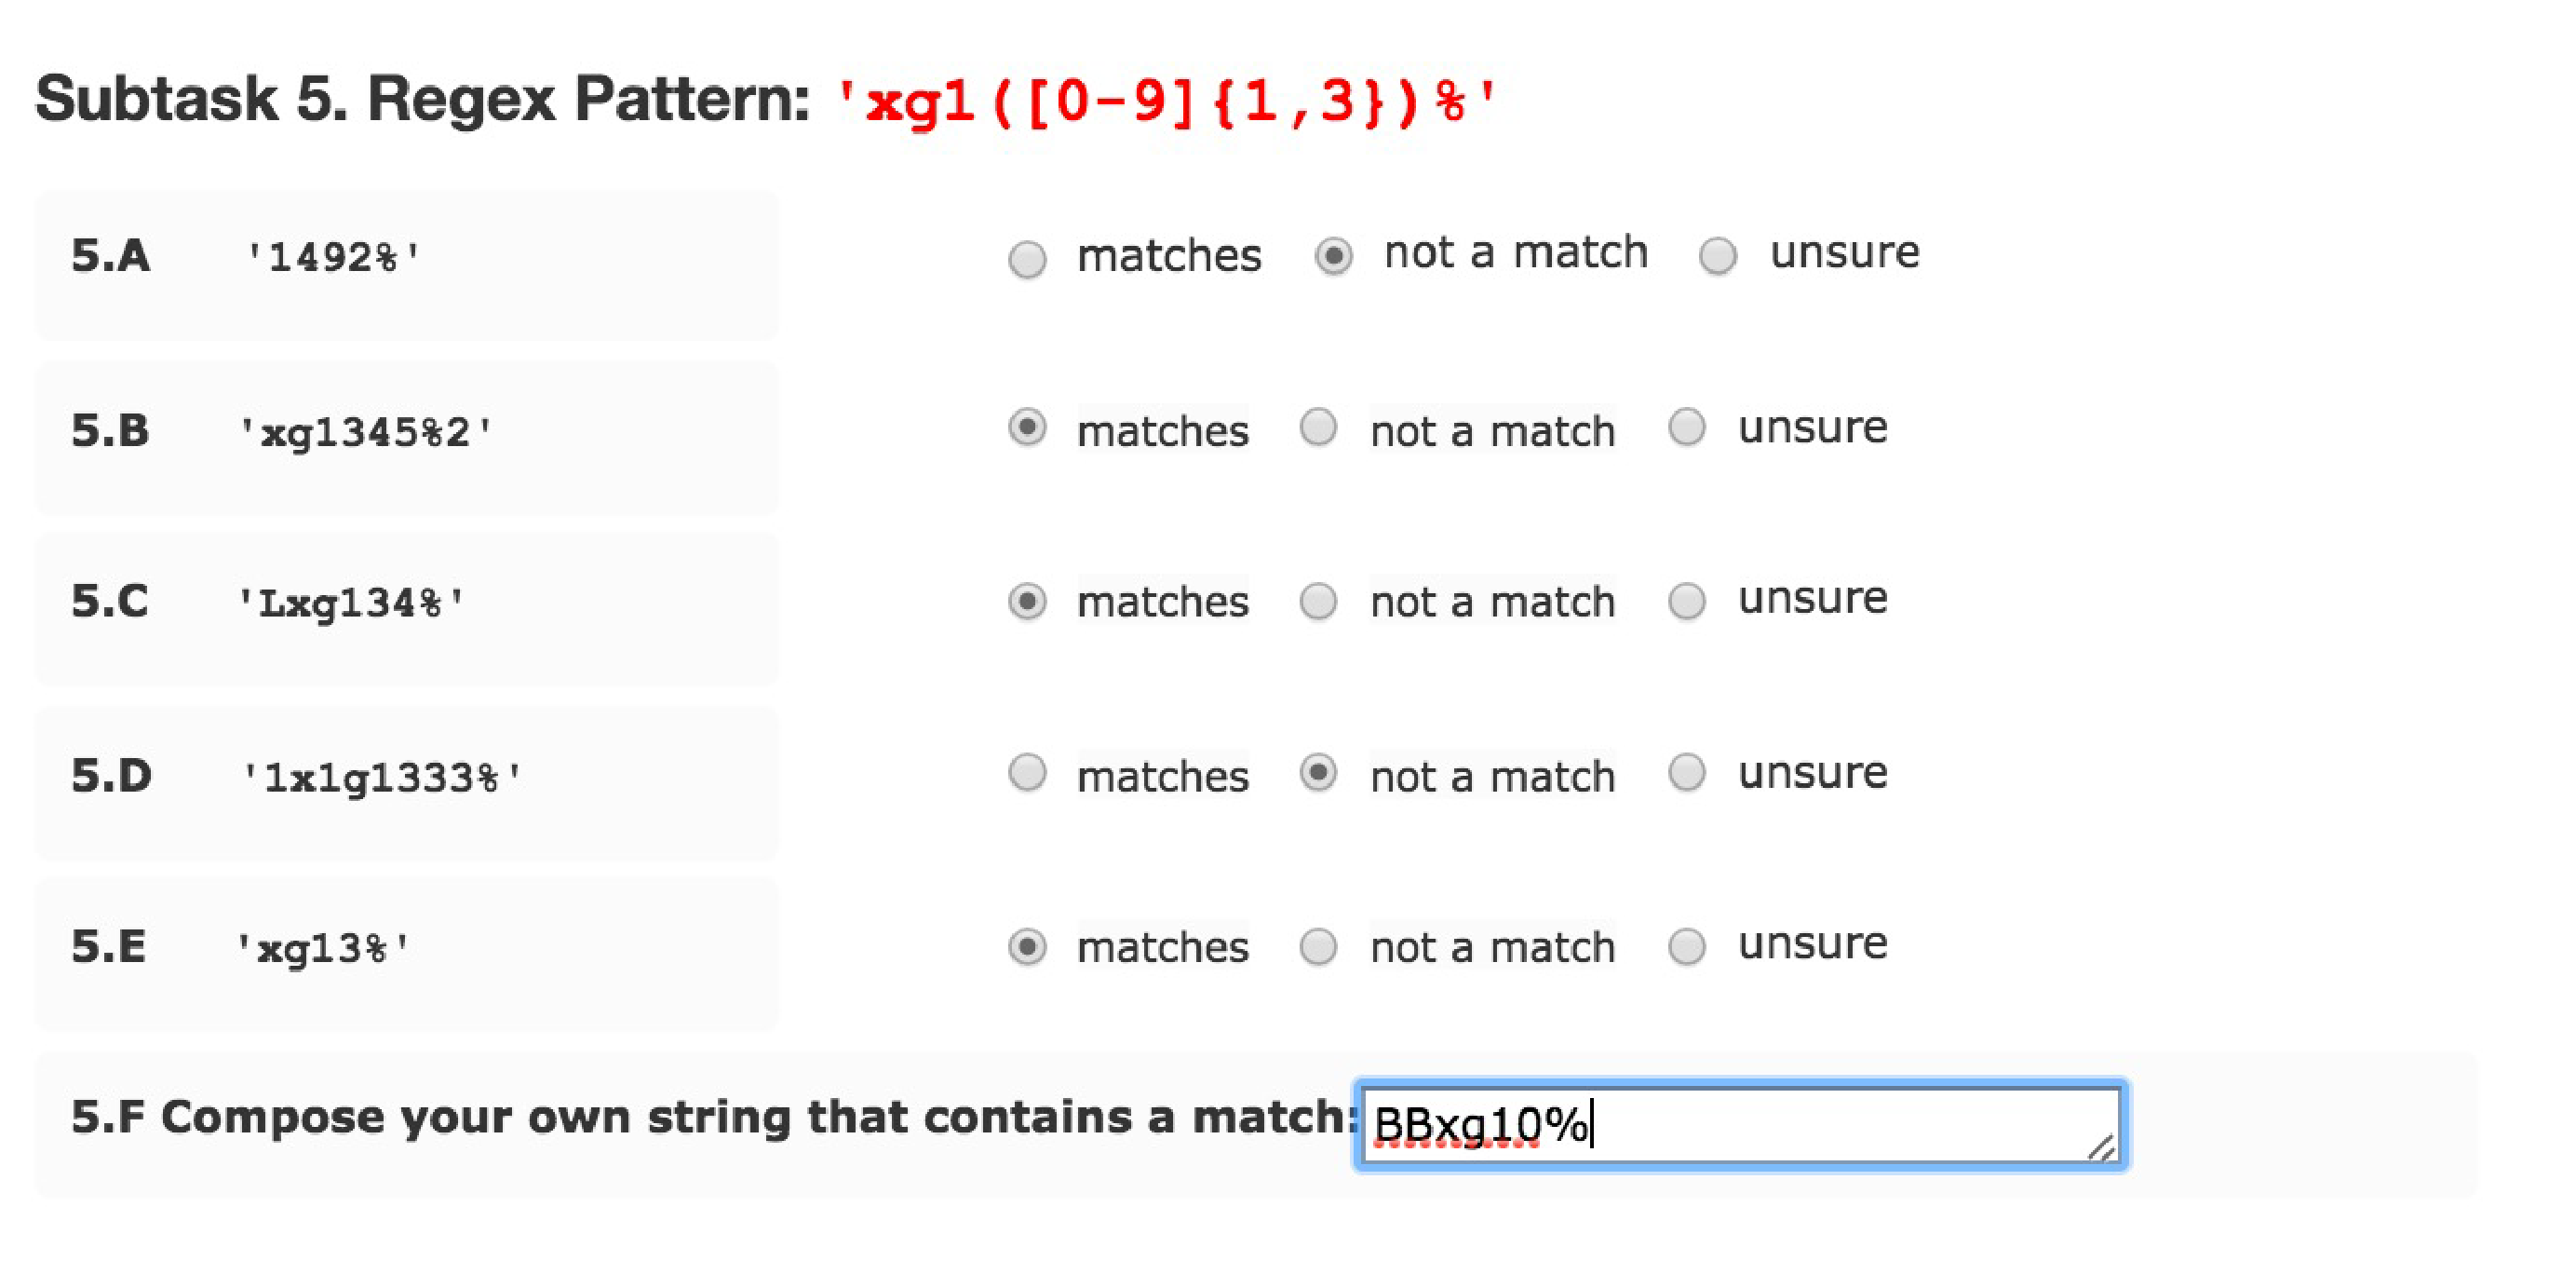
\includegraphics[width=\columnwidth]{illustrations/exampleQuestion}
\vspace{-12pt}
\caption{Example of one HIT Question}
\vspace{-6pt}
\label{fig:exampleQuestion}
\end{figure}

%In Mechanical Turk, we designed a 180 tasks composed of 10 matching subtasks, so that each of the 60 CRs had 30 separate observations (each an average of 5 \emph{example string} problems).  These 1800 observations are what the analysis will focus on. The ordering of the regexes in each HIT was random to control for learning effects.


\begin{table}
\caption{Matching metric example \label{matchingmetric}}
\begin{center}
\begin{small}
\begin{tabular} {cl | c c c c c}
\textbf{String} & \verb!`RR*'! & \textbf{Oracle} & \textbf{P1} & \textbf{P2} & \textbf{P3}& \textbf{P4}\\ \hline
1 & ``ARROW"    & \checkmark    & \checkmark    & \checkmark    & \checkmark    & \checkmark \\
2 & ``qRs"      & \checkmark    & \checkmark    & \xmark        & \xmark        & ?\\
3 & ``R0R"      & \checkmark    & \checkmark    & \checkmark    & ?             & -\\
4 & ``qrs"      & \xmark        & \checkmark    & \xmark        & \checkmark    & -\\
5 & ``98"       & \xmark        & \xmark        & \xmark        & \xmark        & -\\
\hline
  & Score       & 1.00          & 0.80          & 0.80          & 0.50          & 1.00\\
\\
\multicolumn{7}{l}{\checkmark = match, \xmark = not a match, ? = unsure, -- = left blank}\\
\end{tabular}
\end{small}
\end{center}
\end{table}





\subsection{Metrics}
\label{sec:understadningmetric}
 We measure the understandability of regexes using two complementary metrics, \emph{matching} and \emph{compostition}.


\textbf{Matching:}
 Given a regex and a set of strings, a participant determines which strings will be matched by the regex. There are four possible responses for each string, \emph{matches}, \emph{not a match}, \emph{unsure}, or blank. An example from our study is shown in Figure~\ref{fig:exampleQuestion}. 
 
 The percentage of correct responses, disregarding blanks and unsure responses, is the matching score. 
 For example, consider regex \verb!`RR*'! and five strings, which comes from our study, shown in Table~\ref{matchingmetric}, and the responses from four participants in the \emph{P1},\emph{P2},\emph{P3} and \emph{P4} columns. 
 The oracle has the first three strings matching since they each contain at least one \verb!R! character. \emph{P1} answers correctly for the first three strings but incorrectly thinks the fourth string matches, so the matching score is $4/5 = 0.80$. \emph{P2} incorrectly thinks that the second string is not a match, so they also score $4/5 = 0.80$.  \emph{P3} marks `unsure' for the third string and so the total number of attempted matching questions is 4 instead of 5. \emph{P3} is incorrect about the second and fourth string, so they score $2/4 = 0.50$.  For \emph{P4}, we only have data about the first and second matching questions, since the other three are blank.  \emph{P4} marks `unsure' for the second matching question so only one matching question has been attempted, and it was answered correctly so the matching score is $1/1 = 1.00$.
 
Blanks were incorporated into the metric because questions were occasionally left blank in the study. Unsure responses were provided as an option so not to bias the  results when participants were honestly unsure of the answer. These situations did not occur very frequently. Only \todoNow{X\%} of the responses were left blank and only \todoNow{y\%} of the responses were marked as unsure.   


\textbf{Composition:}
Given a regex, a participant composes a string they think it matches. If the participant is accurate and the string indeed is matched by the regex, then a composition score of 1 is assigned, otherwise 0.  For example, given the regex \verb!`(q4fab|ab)'! from our study, the string, ``xyzq4fab" matches  and would get a score of 1, and the string, ``acb" does not match and would get a score of 0.

To determine a match, each regex was compiled using the \emph{java.util.regex} library. A \emph{java.util.regex.Matcher} \verb!m! object was created for each composed string using the compiled pattern.  If \verb!m.find()! returned true, then that composed string was given a score of 1, otherwise it was given a score of 0.



\subsection{Design}
%\todoNow{needs to be updated with respect to no C1,T1 nodes}
This study was implemented on the Amazon's Mechanical Turk (MTurk),  a crowdsourcing platform in which requestors can create human intelligence tasks (HITs) for completion by workers. Each HIT is designed to be completed in a fixed amount of time and workers are compensated with money if their work is satisfactory. Requesters can screen workers by requiring each to complete a qualification test prior to completing any HITs. 

\subsubsection{Worker Qualification}
Workers were pre-qualified by answering questions regarding some basics of regex knowledge. These questions were multiple-choice and asked the worker to describe what the following regexes mean: \verb!a+!, \verb!`(r|z)'!, \verb!`\d'!, \verb!`q*'!, and \verb![p-s]'!. To pass the qualification, workers had to answer four of the five questions correctly.

\subsubsection{Tasks}
Using the regexes in the corpus as a guide, we created 60 regex patterns that were grouped into 26 semantically equivalence groups, where 18 groups had two equivalent regexes each and eight groups had three equivalent regexes each. For example, one of the groups of size two had regexes, \verb!([0-9]+)\.([0-9]+)'! belonging to representation C1 and \verb!(\d+)\.(\d+)'! belonging to representation C4. One of the groups of size thee contained \verb!((q4f)?ab)'! belonging to D2, \verb!(q4fab|ab)'! belonging to D3, and \verb!((q4f){0,1}ab)'! belonging to D1. 
For each of the 26 groups of regexes, we created five strings, where at least two matched and at least two did not match. The fifth string was randomly selected to match or not match. These strings were used to compute the matching metric. 
%These were used for computing the composition metric.

Once all the regexes and matching strings were collected, we created tasks for the MTurk participants as follows: randomly select a regex from ten of the 26 groups. Randomize the order of the regexes, as well as the order of the matching strings for each regex. After adding a question asking the participant to compose a string that the regex matches, this creates one task on MTurk.   This process was completed until each of the 60 regexes appeared in 30 HITs, resulting in a total of 180 HITs.
An example of a single regex, the five matching strings and the space for composing a string is shown in Figure~\ref{fig:exampleQuestion}.


\subsubsection{Implementation}
Workers were paid \$3.00 for successfully completing a HIT, and were only allowed to complete  one HIT. Workers were paid \$3.00 for successfully completing a HIT, and were only allowed to complete  one HIT.  The average completion time for accepted HITs was 682 seconds (11 mins, 22 secs).  A total of 241 HITs were submitted - of those 55 were rejected.
%, and 6 duplicates were ignored, always using the first accepted submission so as to obtain a value for each of the 180 distinct tasks.
Of the 55 rejected HITs, 48 were rushed through by one person leaving many answers blank, 4 other HITs were also rejected because a worker had submitted more than one HIT, one was rejected for not answering composition sections, and one was rejected because it was missing data for 3 questions.  Rejected HITs were returned to MTurk to be completed by others.





\begin{figure}[tp]
\begin{small}
\fbox{\parbox{\columnwidth}{
\begin{enumerate}
\item
\begin{tabular} {lrr}
\textbf{What is your gender?} & \textbf{n} & \textbf{\%}\\ \hline
Male & 149 & 83\%\\
Female & 27& 15\%\\
Prefer not to say & 4& 2\%
\end{tabular}
\item \textbf{What is your age?} \\
$\mu = 31$, $\sigma = 9.3$

\item

\begin{tabular} {l |rr}
\textbf{Education Level?} & \textbf{n} & \textbf{\%}\\ \hline
High School & 5 & 3\%\\
Some college, no degree & 46 & 26\%\\
 Associates degree & 14 & 8\%\\
Bachelors degree & 78 & 43\%\\
Graduate degree & 37 & 21\%\\
\end{tabular}
\item
\begin{tabular} {lrr}
\textbf{Familiarity with regexes?} & \textbf{n} & \textbf{\%}\\ \hline
Not familiar at all & 5 & 3\%\\
Somewhat not familiar & 16 & 9\%\\
Not sure & 2 & 1\%\\
Somewhat familiar & 121 & 67\%\\
Very familiar & 36 & 20\%\\
\end{tabular}
\item \textbf{How many regexes do you compose each year?} \\
$\mu = 67$, $\sigma = 173$
\item \textbf{How many regexes (not written by you) do you read each year?} \\
$\mu = 116$, $\sigma = 275$
%\item In what contexts do you use regexes? \\
\end{enumerate}
}}
\caption{Participant Profiles, $n=180$ \label{participantprofile}}
\end{small}
\end{figure}



\subsection{Participants}

In total, there were 180 different participants in the study.
A majority were male (83\%) with an average age of 31. Most had
at least an Associates degree (72\%) and most were at least somewhat familiar with regexes prior to the study (87\%). On average,
participants compose 67 regexes per year with a range of 0 to 1000. Fittingly, participants read more regexes than they write with an average of 116 and a range from 0 to 2000. Figure~\ref{participantprofile} summarizes the self-reported participant characteristics from the qualification survey.

\begin{table*}\begin{small}\begin{center}\caption{Averaged Info About Edges}\label{table:testedEdgesTable}\begin{tabular}
{llccccccc}
Index & Representations & Pairs & Match1 & Match2 & $H_0: \mu_{match1} = \mu_{match2}$ & Compose1 & Compose2 &  $H_0: \mu_{comp1} = \mu_{comp2}$ \\
\toprule[0.16em]

E8 & C2,T4 -- C5,T1 & 2 & 0.60 & 0.82 & <0.001 & 11.0 & 29.0 & <0.001\\

E16 & T1 -- T4 & 2 & 0.80 & 0.60 & 0.001 & 26.0 & 11.0 & <0.001\\

E5 & C1,T4 -- C2,T1 & 2 & 0.81 & 0.86 & 0.383 & 15.5 & 27.5 & <0.001\\
E4 & C1,T2 -- C2,T1 & 2 & 0.84 & 0.86 & 0.934 & 19.5 & 27.5 & <0.001\\


E12 & D2 -- D3 & 2 & 0.78 & 0.87 & 0.011 & 26.5 & 29.0 & 0.085\\
E13 & L2 -- L3 & 3 & 0.86 & 0.91 & 0.032 & 27.3 & 29.3 & 0.052\\
\hline
E6 & C2 -- C4 & 1 & 0.83 & 0.92 & 0.075 & 18.0 & 20.0 & 0.601\\
E10 & D1 -- D2 & 2 & 0.84 & 0.78 & 0.120 & 28.0 & 26.5 & 0.347\\
E1 & C1 -- C2 & 2 & 0.94 & 0.90 & 0.121 & 28.0 & 27.0 & 0.514\\
E3 & C1 -- C5 & 2 & 0.94 & 0.90 & 0.287 & 28.0 & 28.0 & 1.000\\
E15 & T1 -- T3 & 3 & 0.88 & 0.86 & 0.320 & 21.7 & 22.7 & 0.613\\
E11 & D1 -- D3 & 2 & 0.84 & 0.87 & 0.349 & 28.0 & 29.0 & 0.408\\
E2 & C1 -- C4 & 6 & 0.87 & 0.84 & 0.352 & 25.8 & 25.0 & 0.465\\
E17 & T2 -- T4 & 2 & 0.84 & 0.81 & 0.498 & 19.5 & 15.5 & 0.141\\
E9 & C3 -- C4 & 2 & 0.61 & 0.67 & 0.593 & 22.5 & 24.5 & 0.379\\
E7 & C2 -- C5 & 4 & 0.85 & 0.86 & 0.602 & 26.5 & 28.5 & 0.063\\
E14 & S1 -- S2 & 3 & 0.85 & 0.86 & 0.776 & 26.3 & 27.0 & 0.638\\



\bottomrule[0.13em]\end{tabular}\end{center}\end{small}\end{table*}



\subsection{Analysis}
For each of the 180 HITs, we computed a matching and composition score for each of the 10 regexes, using the metrics described in Section~\ref{sec:understadningmetric}. This allowed us to compute 30 values for each metric and for each of the 60 regexes. Next, we computed average scores for matching and composition per regex. 

Each regex was a member of one of 26 groupings of equivalent regexes. These groupings allow pairwise comparisons of the metrics values to determine which representation of the regex was most understandable. Among all the groups, we performed 42 pairwise comparisons of the matching and composition scores  (i.e., one comparison for each group of size two and three comparisons within each group of size three). 
For example, one group of size two had regexes, \verb!RR*! and \verb!R+!, which are equivalent and represent a transformation between L2 and L3. The former had an average matching of \todoNow{X} and the latter had an average matching of \todoNow{Y}. The average composition score for the former was \todoNow{Z} and \todoNow{W} for the latter. Thus, the community found \todoNow{state the regex} from representation \todoNow{L?} more understandable. There were two other pairwise comparisons performed between the L2 and L3 group, using regexes pair \verb!zaa*! and \verb!za+'!, and regexes pair \verb!\..*! and \verb!\.+'!. Considering all three of these regex pairs, the overall matching average for the regexes belonging to L2 was 0.86 and 0.91 for L3. The overall composition score for L2 was 0.91 and 0.98 for L3. Thus, the community found L3 to be more understandable, from the perspective of both understandability metrics, than L2. 
This information is presented in summary in Table~\ref{table:testedEdgesTable}, with this specific example appearing in the E3 row. The \emph{Index} column enumerates all the pairwise comparisons evaluated in this experiment, \emph{Representations} lists the two representations, \emph{Pairs} shows how many comparisons were performed, \emph{Match1} gives the overall matching score for the first representation listed, \emph{Match2} gives the overall matching score for the second representation listed, and $H_0: \mu_{match1} = \mu_{match2}$ uses the Mann-Whitney test of means to compare the matching scores, and presents the p-values. The last three columns list the average composition scores for the representations and the p-value, also using the Mann-Whitney test of means. 

%60 strings
%42 comparisons
%18@2, 8@3
%
%M6R1 ? group 3, 3 comparisons
%- 1 comparisons
%- 0 strings
%
%M3R0 ? group 3, 3 comparisons
%- 1 comparisons
%- 0 strings
%
%M3R1 ? group 3, 3 comparisons
%- 2 comparisons
%- 1 string
%
%M3R0 ? group 3, 3 comparisons
%- 2 comparisons
%- 1 string
%
%58 strings
%36 comparisons 


Although we had 42 pairwise comparisons,  we had to drop six comparisons  due to a design flaw since the regex examples performed transformations from multiple equivalence classes. For example, regex \verb!([\072\073])! is in C2 and T4, and was grouped with regex \verb!(:|;)! in C5, T1, so it was not clear if any differences in understandability were due to the transformation between C2 and C5, or T4 and T1. However, the third member of the group, \verb!([:;])!, could be compared with both, since it is a member of T1 and C2, so comparing it to \verb!([\072\073])! evaluates the transformation between T1 and T4, and comparing to \verb!(:|;)! evaluates the transformation between C2 and C5. The end result is 36 pairwise comparisons across 14 edges from Figure~\ref{fig:refactoringTree}. 


%For each of the 60 regexes, an average matching score was computed using the metrics in Table~\ref{matchingmetric}. The average composition metric was measured using the process described in Section~\ref{sec:metric}. This addresses \emph{RQ2} and \emph{RQ3}.

%\todoNow{How to deal with unsure responses? How many were there? Carl's analysis goes here.}



\subsection{Results}
Table~\ref{table:testedEdgesTable} presents the results of the understandability analysis. A horizontal line separates the first three edges from the bottom 11. In E1 through E3, there is a statistically significant difference between the representations for at least one of the metrics considering $\alpha = 0.05$.  These represent the strongest evidence for suggesting refactoring based on the understandability metrics we defined. Specifically, T4 $\Rightarrow$ T1, D2 $\Rightarrow$ D3, and L2 $\Rightarrow$ L3 are likely to improve understandability. 

We note here that participants were able to select \emph{unsure} when they were not sure if a string would be matched by a regex (Figure~\ref{fig:exampleQuestion}). From a comprehension perspective, this indicates some level of confusion and we can use that to further corroborate the understandability analysis. 

\todoNow{incorporate unsure analysis here}




\section{Understandability Study (RQ1)}
\label{sec:rq1}
This study presents programmers with regexes and asks comprehension questions. By comparing the understandability of semantically equivalent regexes that match the same language but have different syntactic representations, we aim to identify understandability code smells.
This study was implemented on Amazon's Mechanical Turk with 180 participants. A total of 60 regexes were evaluated, constructing 42 pairs of regex comparison. Each regex pattern was evaluated by 30 participants.
%The patterns used were designed to belong to various representations in Figure~\ref{fig:refactoringTree}.







\subsection{Metrics}
\label{sec:understadningmetric}
 We measure the understandability of regexes using two complementary metrics, \emph{matching} and \emph{composition}. These are referred to as the \emph{comprehension metrics}.
For a deeper look at the data to gain a better understanding of factors that impact comprehension, we also compute \emph{regex length} and \emph{DFA size} for each regex.


\textbf{Matching:}
 Given a pattern and a set of strings, a participant determines by inspection which strings will be matched by the pattern. There are four possible responses for each string, \emph{matches}, \emph{not a match}, \emph{unsure}, or blank. An example\footnote{Task instructions are also available: \url{https://github.com/wangpeipei90/RegexSmells/blob/master/questionnaire.pdf}} from our study is shown in Figure~\ref{fig:exampleQuestion}.

 The percentage of correct responses, disregarding blanks and unsure responses, is the matching score.
 For example, consider regex pattern \verb!`RR*'!, the five strings shown in Table~\ref{matchingmetric}, and the responses from four participants in the \emph{P1}, \emph{P2}, \emph{P3} and \emph{P4} columns.
 The {\em Oracle} indicates the first three strings match and the last two do not; 
 %Python's {\tt  re.search()} function is used to determine a match. 
 \emph{P1} answers correctly for the first three strings and the fifth, but incorrectly on the fourth, so the matching score is $4/5 = 0.80$. \emph{P2} incorrectly thinks that the second string is not a match, so the score is also $4/5 = 0.80$. \emph{P3} marks `unsure' for the third string and so the total number of attempted matching questions is 4. \emph{P3} is incorrect about the second and fourth string, so they score $2/4 = 0.50$. For \emph{P4}, we only have data for the first and second strings, since the other three are blank. \emph{P4} marks `unsure' for the second string so only one matching question has been attempted; the matching score is $1/1 = 1.00$.

Blanks were incorporated into the metric because questions were occasionally left blank in the study. Unsure responses were provided as an option so not to bias the results through blind guessing. These situations did not occur very frequently.
%Only 1.1\% of the responses were left blank and only 3.8\% of the responses were marked as unsure. %We refer to a response with all blank or unsure responses as an `NA'.
Out of 1,800 questions (180 participants * 10 questions each), only 1.8\%(32) were impacted by a blank or unsure response (never more than four out of 30 responses per pattern).


\begin{figure}[tb]
\centering
%\includegraphics[width=0.75\columnwidth]{illustrations/ExampleQuestion}
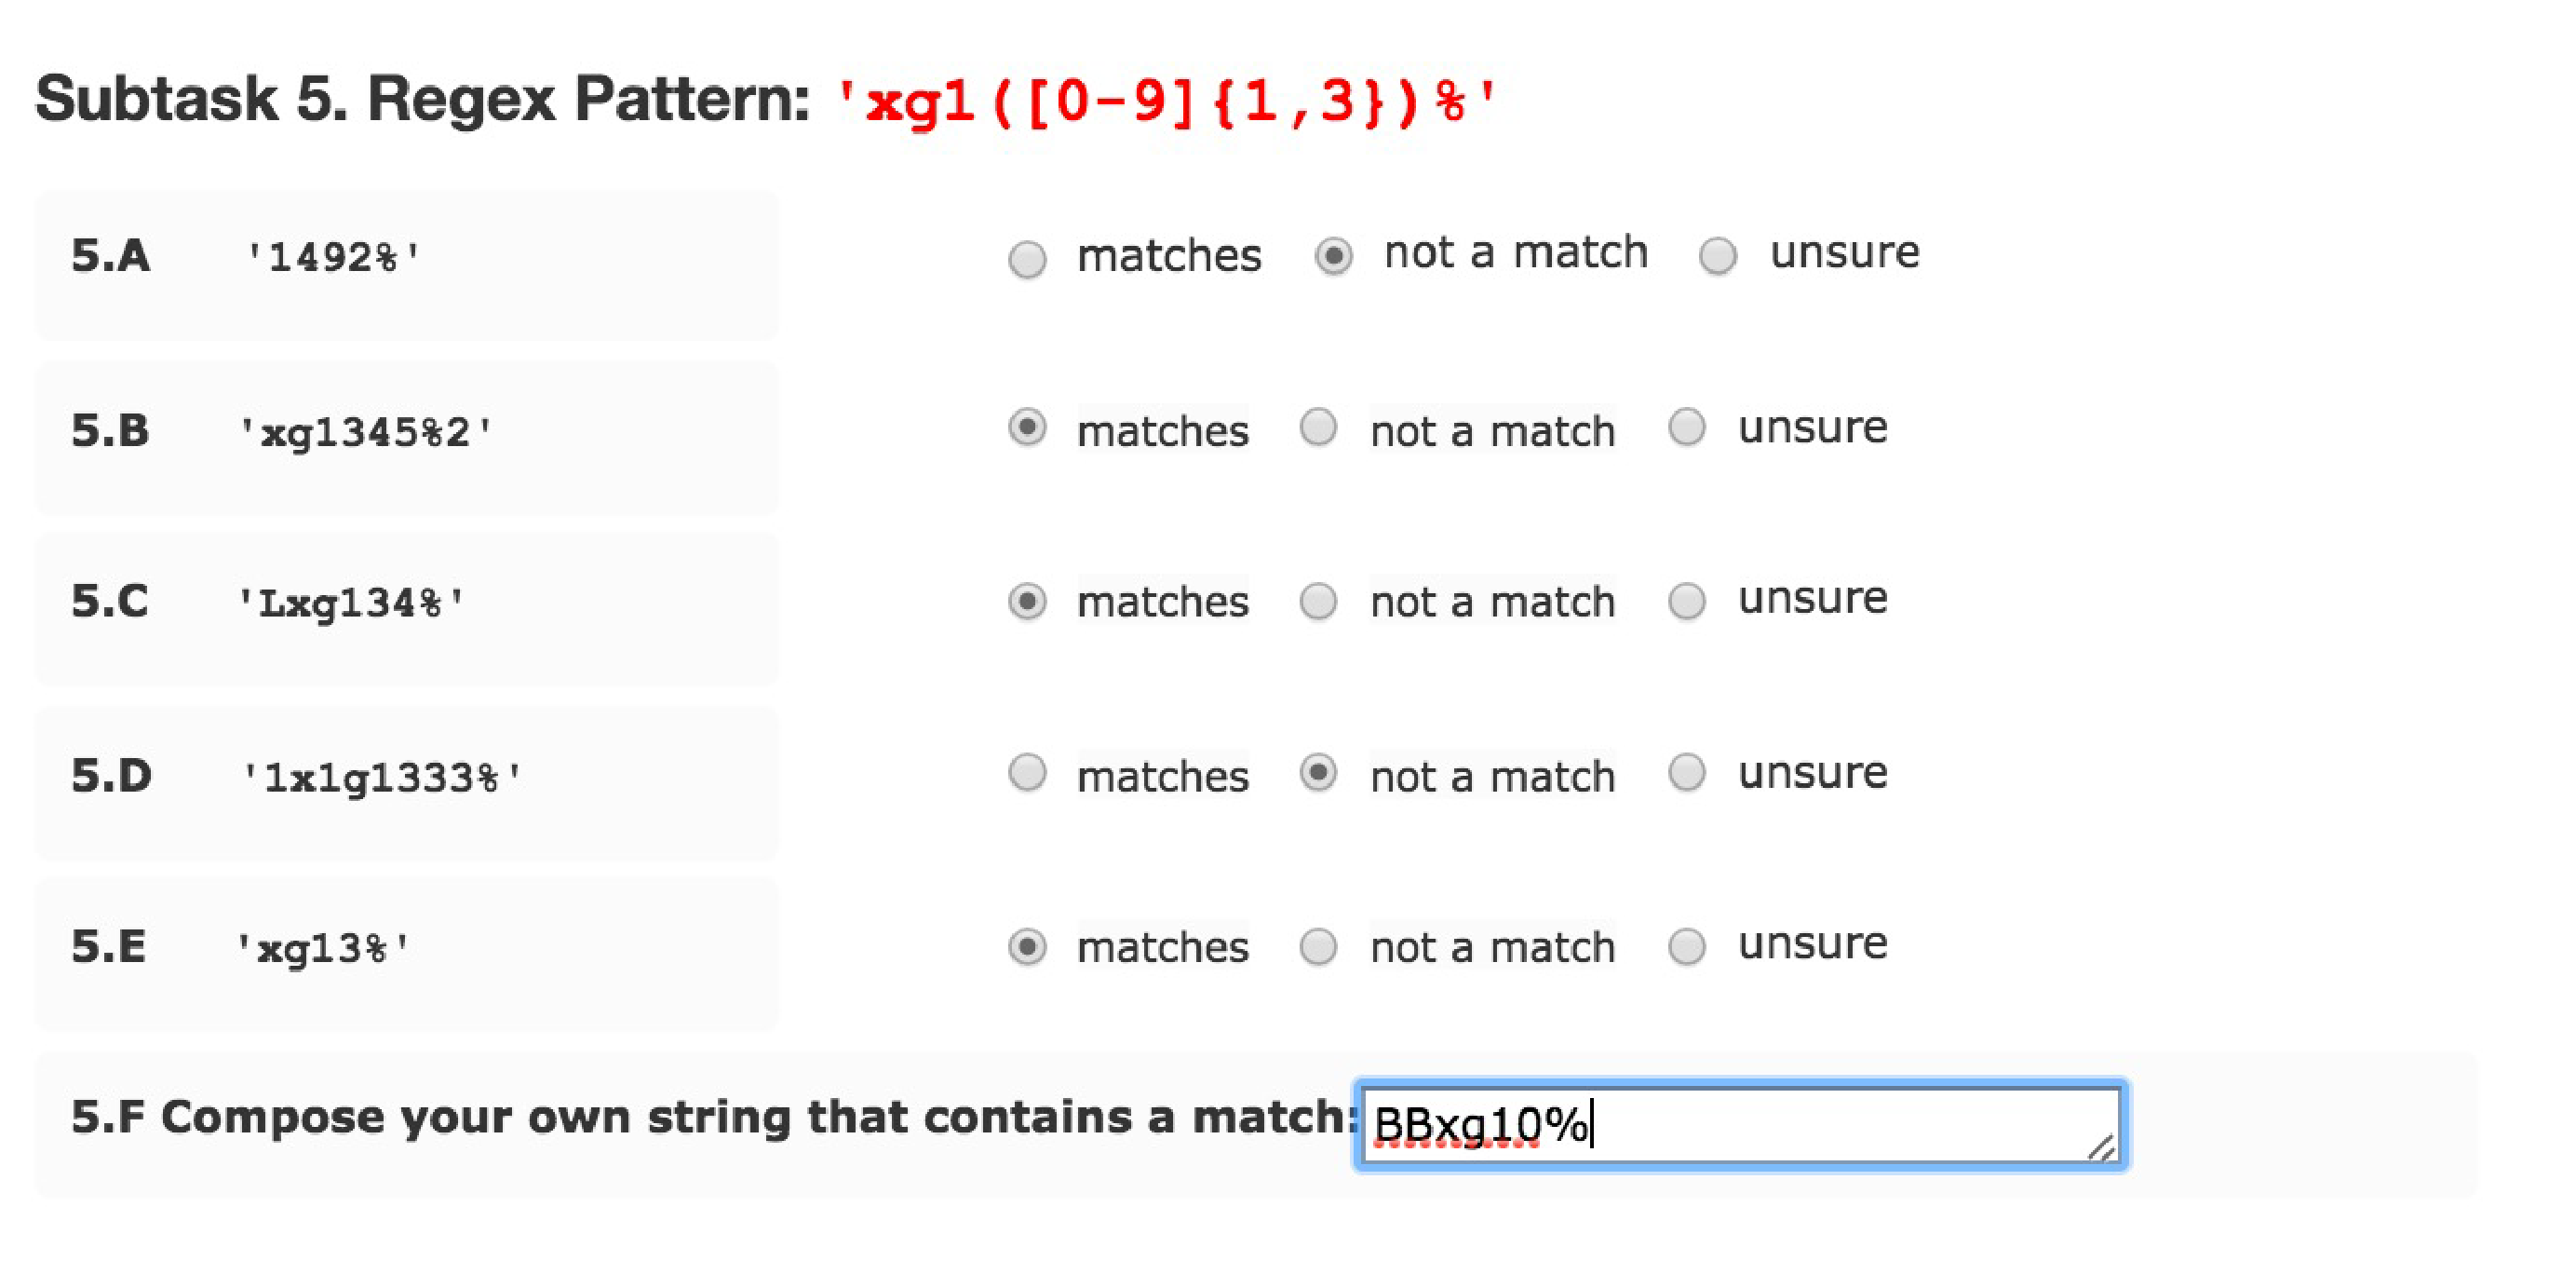
\includegraphics[width=0.75\columnwidth]{illustrations/exampleQuestion.eps}
\vspace{-3pt}
\caption{Questions from one pattern in one HIT}
\vspace{-6pt}
%\vspace{-6pt}
\vspace{-3pt}
\label{fig:exampleQuestion}
\end{figure}



\begin{table} [t]
\vspace{2mm}
\caption{Matching metric example \label{matchingmetric}}
\vspace{-12pt}
\begin{center}
%\begin{small}
%\vspace{-6pt}
\begin{tabular} {|cl | c c c c c|} \hline
\textbf{String} & \verb!`RR*'! & \textbf{Oracle} & \textbf{P1} & \textbf{P2} & \textbf{P3}& \textbf{P4}\\ \hline
1 & ``ARROW"    & \checkmark    & \checkmark    & \checkmark    & \checkmark    & \checkmark \\
2 & ``qRs"      & \checkmark    & \checkmark    & \xmark        & \xmark        & ?\\
3 & ``R0R"      & \checkmark    & \checkmark    & \checkmark    & ?             & -\\
4 & ``qrs"      & \xmark        & \checkmark    & \xmark        & \checkmark    & -\\
5 & ``98"       & \xmark        & \xmark        & \xmark        & \xmark        & -\\
\hline
  & Score       & 1.00          & 0.80          & 0.80          & 0.50          & 1.00\\ \hline
%\multicolumn{7}{l}{}\\
\multicolumn{7}{l}{\checkmark = match, \xmark = not a match, ? = unsure, -- = left blank}\\
\end{tabular}
%\vspace{-6pt}
\vspace{-6pt}
%\end{small}
\end{center}
\vspace{-6pt}
%\vspace{-6pt}
\vspace{-3pt}
\end{table}



\textbf{Composition:}
Given a pattern, a participant composes a string they think it matches (question 7.F in Figure~\ref{fig:exampleQuestion}). If the participant is accurate, a composition score is 1, otherwise 0. For example, given the pattern \verb!(q4fab|ab)! from our study, the string, ``xyzq4fab" matches and gets a score of 1, but the string, ``acb" does not match and gets a score of 0.

%To determine a match, each pattern was compiled using the \emph{java.util.regex} library. A \emph{java.util.regex.Matcher} \verb!m! object was created for each composed string using the compiled pattern. If \verb!m.find()! returned true, then that composed string was a match and scored 1, otherwise it scored 0.
%To determine a match, each pattern was compiled using the \emph{java.util.regex} library in Java. A {\em java.util.regex.Matcher} \verb!m! was created for each composed string using the compiled pattern. If {\tt m.find()} returns {\tt true}, then that composed string was a match and scored 1; otherwise it scored~0.

%To determine a match, each pattern was compiled using the \emph{re.compile} module in Python. A regular expression object \verb!m! was created using the compiled pattern. \verb!m.search()! returns a regular match object \verb!m2! with the composed string as the input of the function. If \verb!m2! is not \emph{None}, then that composed string was a match and scored 1; otherwise it scored~0.
To determine the match between a string and a pattern, the pattern is compiled using the \emph{re.compile} module in Python. An instance of \emph{re.RegexObject} \verb!m! is created using the compiled pattern. \emph{m.search()} returns an instance of \emph{re.MatchObject} \verb!m2! with the string given as the input to this function. If \verb!m2! is not \emph{None}, then that string was a match and scored 1; otherwise it scored~0.


\textbf{Regex Length:}
Given a pattern, the regex length is computed by its literal string length. For example, regexes \verb!\072! and \verb!ab*c! are both length four.


\textbf{DFA Size:}
Given a pattern,To compute the size of minimal DFA, we run both \textit{brics}~\cite{brics} and \textit{Rex}~\cite{rex} on each regex, and manually check their results to guarantee their correctness.
%The DFA size is the number of states of minimal DFA. We run both \textit{brics}~\cite{brics} and \textit{Rex}~\cite{rex} on each regex in order to get the minimal DFA. We also mannually check their results to guarantee their correctness.
\iffalse
We note that \textit{brics} always shows the minimal DFAs but its syntax is very restricted in language coverage~\cite{chapman2016} while \textit{Rex} accepts most regular expression features, but does not guarantee a minimal DFA (although, as it turns out, most are minimal). %Although most of the DFAs generated by \textit{Rex} are minimal but they are not guaranteed to be minimal.
For the regexes that are accepted by both \textit{brics} and \textit{Rex}, we chose the size of DFA generated from \textit{brics}. For example, the DFA size got from \textit{brics} for {\tt RR*} is two while the size from \textit{Rex} is three; thus, we select the smaller one.
For the regexes only accepted by \textit{Rex}, we examined the generated DFAs manually and made minor changes to make sure we use the minimal one. {\tt tuv$\backslash$w} and {\tt [a-f]($\backslash$d+)[a-f]} are only accepted by \textit{Rex} because {\tt $\backslash$w} and {\tt $\backslash$d} are not valid in \textit{brics}. While the DFA sizes for both regexes from \textit{Rex} are five, we set the DFA size of {\tt tuv$\backslash$w} to five and the DFA size of {\tt [a-f]($\backslash$d+)[a-f]} to four. This is because the DFA of the former is minimal but that of the latter is not minimal and could be reduced.
\fi
\subsection{Design}
%\todoNow{needs to be updated with respect to no C1,  T1 nodes}
We implemented this study on Amazon's Mechanical Turk (MTurk), a crowdsourcing platform where requesters create human intelligence tasks (HITs) for completion by workers.
%Each HIT is designed to be completed in a fixed amount of time and workers are compensated with money if their work is satisfactory. Requesters can screen workers by requiring each to complete a qualification test prior to completing any HITs.

%\subsubsection{Worker Qualification}
\textbf{Worker Qualification:}
Qualified workers had to answer four of the five basic regex questions correctly. These questions were multiple-choice and asked the worker to analyze the following patterns: \verb!a+!, \verb!(r|z)!, \verb!\d!, \verb!q*!, and \verb![p-s]!.
% To pass the qualification test, workers had to answer four of the five questions correctly.
%\subsubsection{Tasks}

\textbf{Tasks:}
Guided by the patterns in the corpus, we created 60 regex patterns that were grouped into 26 semantic equivalence groups. 
There were 18 groups with two regexes targeting various edges in the equivalence classes. The other eight groups had three regexes each. In total there are 42 pairs of patterns. 
%These semantic groups were intended to explore edges in the equivalence classes. 
In this way, we can draw conclusions by comparing representations since the regexes evaluated were semantically equivalent.

To form the semantic groups, we took a regex from the corpus, matched it to a representation in Figure~\ref{fig:refactoringTree}, trimmed it down so it contained little more than just the feature of interest, and then created other regexes that are semantically equivalent but belong to other nodes in the equivalence class. For example, a semantic group with regexes \verb!((q4f){0,1}ab!, \verb!((q4f)?ab)!, and \verb!(q4fab|ab)! belong to D1, D2, and D3, respectively.
A group with regexes \verb!([0-9]+)\.([0-9]+)! and \verb!(\d+)\.(\d+)! is intended to evaluate the edge between C1 and C4.
We note that if we only used regexes from the corpus, we would have had regexes with different semantics at each node, or with additional language features, which would make the comparisons of the targeted features difficult.
\\
For each of the 26 semantic groups, we created five strings for the study, where at least one matched and at least one did not match. These were used to compute the matching metric.
\\
Once all the patterns and matching strings were collected, we created tasks for the MTurk participants as follows:
randomly select a pattern from 10 of the 26 semantic groups. Randomize the order of these 10 patterns, as well as the order of the matching strings for each pattern. After adding a question asking the participant to compose a string that each pattern matches, this creates one task on MTurk, such as the example in Figure~\ref{fig:exampleQuestion}. This process was completed until each of the 60 regexes appeared in 30 HITs, resulting in a total of 180 total unique HITs.
%An example of a single regex pattern, the five matching strings and the space for composing a string is shown in
%\subsubsection{Implementation}

\textbf{Implementation:}
Workers were paid \$3.00 for successfully completing one and only one HIT. The average completion time for accepted HITs was 682 seconds (11 mins, 22 secs).
%A total of 241 HITs were submitted - of those 55 were rejected.
% and 6 duplicates were ignored, always using the first accepted submission so as to obtain a value for each of the 180 distinct tasks.
A total of 54 HITs were rejected: 48 had too many blank responses, four were double-submissions by same workers, one did not answer composition questions, and one missed data of 3 questions. Rejected HITs were returned to MTurk to be completed by others.
%\subsubsection{Participants}

\textbf{Participants:}
In total, there were 180 participants.
A majority were male (83\%). % with an average age of 31.
Most had
at least an Associates degree (72\%), were at least somewhat familiar with regexes (87\%), and had prior programming experience (84\%).
%On average,
%participants compose 67 regexes per year with a range from 0 to 1000.
%Participants read more regexes than they write with an average of 116 and a range from 0 to 2000.
%Figure~\ref{participantprofile} summarizes the self-reported participant characteristics from the qualification survey.


%\todoNow{in study section present choices about pairwise vs random selection for nodes.}



\begin{table}[t]
\vspace{2mm}
\centering
\caption{3-factor ANOVA with average matching or composition accuracy as dependent variables, considering representation (rep), DFA size (dfa\_size), and regex length (len) as independent variables}
\vspace{-3pt}
\begin{tabular}{@{}l@{}r|rl|ll@{}}

  \multicolumn{2}{c}{} & \multicolumn{2}{c}{Average Matching} & \multicolumn{2}{c}{Average Composition} \\
    \hline
 & Df & F value & Pr($>$F) & F value & Pr($>$F) \\
  \hline
dfa\_size &              1 &  7.632 &0.0153 * & 10.084 &0.00674 ** \\
len      &          1 &  3.325 &0.0896 $\cdot$ &  0.001 &0.98161 \\
rep            &      15 &  2.062 &0.0921 $\cdot$ & 1.224 &0.35538\\
dfa\_size:len  &     1 & 1.002 &0.3339  & 1.384 &0.25907   \\
dfa\_size:rep    &     14 & 0.709 &0.7355 &0.920& 0.56075   \\
len:rep     &     10 & 0.924& 0.5397  &  0.599& 0.79054   \\
dfa\_size:len:rep  &3&  1.163& 0.3589 & 0.678 &0.58002   \\
Residuals        &     14&&&&\\
   \hline
\end{tabular}

\vspace{3pt}
$\cdot\alpha = 0.10$ \hspace{3pt} *$\alpha=0.05$ \hspace{3pt} **$\alpha=0.01$ \hspace{3pt} ***$\alpha=0.001$
%The F values and p values in column 3-4 are of ANOVA results with average matching accuracy as dependent variables. These values in column 5-6 are for ANOVA results with composition accuracy.

\label{table:anova}
\vspace{-6pt}
\vspace{-3pt}
%\vspace{-3pt}
\end{table}

\iffalse
\begin{table}[t]
\centering
\caption{3-factor ANOVA results with average composition accuracy as the dependent variable, considering representation (rep), DFA size (dfa\_size), and regex length (len) as independent variables}
\begin{tabular}{@{}l@{}rrrrl@{}}
  \hline
 & Df & Sum Sq & Mean Sq & F value & Pr($>$F) \\
  \hline
dfa\_size     &          1 &  3548 &   3548 & 10.084 &0.00674 **\\
len     &           1    &  0    &   0 &  0.001 &0.98161 \\
rep              &    15   &6458  &   431  & 1.224 &0.35538\\
dfa\_size:len   &    1   & 487   &  487  & 1.384 &0.25907   \\
dfa\_size:rep     &    14  & 4532    & 324   &0.920& 0.56075   \\
len:rep     &     10  & 2107&     211 &  0.599& 0.79054   \\
dfa\_size:str:rep & 3  &  715 &    238  & 0.678 &0.58002   \\
Residuals          &   14  & 4926  &   352  &&\\
   \hline
\end{tabular}

\vspace{3pt}
.$\alpha = 0.10$ \hspace{3pt} *$\alpha=0.05$ \hspace{3pt} **$\alpha=0.01$ \hspace{3pt} ***$\alpha=0.001$
\label{table:anova2}
\end{table}
\fi

\begin{table*}\begin{small}\begin{center}\caption{Averaged Info About Edges}\label{table:testedEdgesTable}\begin{tabular}
{llccccccc}
Index & Representations & Pairs & Match1 & Match2 & $H_0: \mu_{match1} = \mu_{match2}$ & Compose1 & Compose2 &  $H_0: \mu_{comp1} = \mu_{comp2}$ \\
\toprule[0.16em]

E8 & C2,T4 -- C5,T1 & 2 & 0.60 & 0.82 & <0.001 & 11.0 & 29.0 & <0.001\\

E16 & T1 -- T4 & 2 & 0.80 & 0.60 & 0.001 & 26.0 & 11.0 & <0.001\\

E5 & C1,T4 -- C2,T1 & 2 & 0.81 & 0.86 & 0.383 & 15.5 & 27.5 & <0.001\\
E4 & C1,T2 -- C2,T1 & 2 & 0.84 & 0.86 & 0.934 & 19.5 & 27.5 & <0.001\\


E12 & D2 -- D3 & 2 & 0.78 & 0.87 & 0.011 & 26.5 & 29.0 & 0.085\\
E13 & L2 -- L3 & 3 & 0.86 & 0.91 & 0.032 & 27.3 & 29.3 & 0.052\\
\hline
E6 & C2 -- C4 & 1 & 0.83 & 0.92 & 0.075 & 18.0 & 20.0 & 0.601\\
E10 & D1 -- D2 & 2 & 0.84 & 0.78 & 0.120 & 28.0 & 26.5 & 0.347\\
E1 & C1 -- C2 & 2 & 0.94 & 0.90 & 0.121 & 28.0 & 27.0 & 0.514\\
E3 & C1 -- C5 & 2 & 0.94 & 0.90 & 0.287 & 28.0 & 28.0 & 1.000\\
E15 & T1 -- T3 & 3 & 0.88 & 0.86 & 0.320 & 21.7 & 22.7 & 0.613\\
E11 & D1 -- D3 & 2 & 0.84 & 0.87 & 0.349 & 28.0 & 29.0 & 0.408\\
E2 & C1 -- C4 & 6 & 0.87 & 0.84 & 0.352 & 25.8 & 25.0 & 0.465\\
E17 & T2 -- T4 & 2 & 0.84 & 0.81 & 0.498 & 19.5 & 15.5 & 0.141\\
E9 & C3 -- C4 & 2 & 0.61 & 0.67 & 0.593 & 22.5 & 24.5 & 0.379\\
E7 & C2 -- C5 & 4 & 0.85 & 0.86 & 0.602 & 26.5 & 28.5 & 0.063\\
E14 & S1 -- S2 & 3 & 0.85 & 0.86 & 0.776 & 26.3 & 27.0 & 0.638\\



\bottomrule[0.13em]\end{tabular}\end{center}\end{small}\end{table*}


\subsection{Analysis}
We computed a matching and composition score for each regex based on the 30 participant responses.
The average analysis or average composition is computed by averaging the associated 26-30 values for each metric for each of the 60 regexes (fewer than 30 values were used if all the responses in a matching question were a combination of blanks and unsure). %Next, we computed average scores for matching and composition per regex.
%\todoLast{Mentioning NAs here?}


%Each regex was a member of one of 26 groupings of equivalent regexes.
%These groupings allow pairwise comparisons of the metrics values to determine which representation of the regex was most understandable and the direction of a refactoring for understandability.
Of the original 42 pairs, we report scores for 41. Due to a design flaw, the regexes evaluated, \verb!\..*! and \verb!\.+!. were not semantically equivalent (the former is missing an escape and should be \verb!\.\.*!), so this was omitted from the data. In the end, we analyzed 58 regexes that cover 17 edges from Figure~\ref{fig:refactoringTree}.

To gain a better understanding of why some regexes may be more understandable than others, we also look at the impact of the representation from Figure~\ref{fig:refactoringTree}, regex length, and DFA size\footnote{Note that the study was not specifically designed for regex length and DFA size} on the comprehension metrics.
Note that we retain all 60 regexes for this analysis as we are looking at the properties of regexes individually.
We conduct two three-factor analysis of variances (ANOVAs) with matching accuracy and composition accuracy as the dependent variables.
We also conduct the correlation analysis between these three factors and the composition metrics.
We use Spearman's Rank-Order Correlation because we have no priori knowledge about the distributions of the factors.
Since the regex representations are categorical data, these are excluded from the correlation analysis.



\subsection{Results}
The ANOVA in Table~\ref{table:anova} shows that DFA size significantly affects both the average matching accuracy and the average composition at $\alpha = 0.05$ and $\alpha = 0.01$, respectively.
The length and representation from Figure~\ref{fig:refactoringTree} each significantly affect the average matching accuracy at $\alpha = 0.10$.
Since the DFA sizes vary across the pairwise comparisons within a representation, we present our results for matching and composition using each of the 41 pairs of regexes separately, rather than in aggregate over the equivalence class edges explored. %

%\textcolor{red}{Todo: update Table and its description, add annova and correlation analysis about representation, dfa size, and string length}

For the comprehension metrics, Table~\ref{table:testedEdgesTable} presents the results.
Each row represents a {\em Pair} of regex evaluated by study participants.
The representations for the regexes per Figure~\ref{fig:refactoringTree} are shown in the {\em Edge} column, which is how the table is sorted.
The {\em Regex 1} and {\em Regex 2} columns identify the regexes used in the study, mapping to the first and second representations in the {\em Edge} column, respectively.
{\em Match1} is the average matching for {\em Regex 1} and {\em Match2} is the average matching for {\em Regex~2}.
Using the Mann-Whitney test of means, the {\em sigM} column following tests if there is a significant difference between the accuracies.
The {\em Comp1} column presents the percentage of the string responses for that were in fact correctly matched by {\em Regex 1}. {\em Comp2} presents the same information, except for {\em Regex 2}.
The following {\em sigC} column uses a test of two proportions to identify if the percentage of the participants who correctly composed a string for Regex 1 is significantly different than the percentage who correctly composed a string for {Regex 2}.

%, \emph{Nodes} lists the representations, \emph{Pairs} shows the number of comparisons, \emph{Example Preferred Regex} shows a regex from the preferred node (bolded in \emph{Pairs} column), \emph{Match1} and \emph{Match2} give the matching scores for the first and second representations, respectively, and $H_0: \mu_{match1} = \mu_{match2}$ uses the Mann-Whitney test of means to compare the matching scores, and presents the p-values. The last three columns list the average composition scores for the representations and the composition p-value.

To illustrate, consider pair 16 in Table~\ref{table:testedEdgesTable}.
One pair of regexes was \verb!([}{])! and \verb!(\{|\})! in C4 and C5, respectively, with average matching scores of 78.79\% and 70.33\% and average composition scores of 50.00\% and 86.67\%, respectively.
The difference between the composition scores is significant at $\alpha = 0.01$, yet the difference between the accuracies is not.
In fact, the representation C5 was more understandable in that participants could more effectively compose a string that it would match, but C4 is more understandable in that participants could more easily determine which of a set of strings would be matched by C4. Thus, neither representation is bolded in the \emph{Edge} column since there is a conflict.
If both comprehension metrics indicated a preferred representation, that representation is bolded (e.g., C4 in pair 15). Ties are broken by deferring to the other metric. For example, there's a tie in composition for pair 17, but matching indicates a preference for C5. Therefore C5 is bolded.

For pairs 16, 29, 34, and 36, the difference in composition is significant at $\alpha < 0.05$, indicating differences favoring C5 over C4, T1 over T2, and twice favoring T1 over T4.
For pairs 23, 37, and 38, the difference in matching is significant with $\alpha < 0.05$, indicating differences favoring D3 over D2 and twice favoring T1 over T4.
%There appears to be a clear trend favoring T1 over T4.
Interestingly, for pairs 16 and 29, while the differences in composition are significant, there is a conflict between the composition metrics. Further investigation is needed to understand in what circumstances the metrics are in conflict with one another.
% and we can use that to further corroborate the understandability analysis.
%\begin{table*}
%\centering
%\caption{Average Unsure Responses Per Pattern By Node (fewer unsures on the left)}\label{table:unsureResults}
%\begin{tabular}{|| l || cccc || cccc || || cccc || cccc ||}
%                & \multicolumn{4}{c||}{>=Q0(0.67)}         & \multicolumn{4}{c||||}{>=Q1(1.25)}   & \multicolumn{4}{c||}{>=Q2(1.94)}    &  \multicolumn{4}{c||}{>=Q3(2.54)}  \\ \hline
%Node     & L3 & D3 & C2 & C1 & L2 & S2 & S1 & C4 & D1 & C5 & C3 & D2 & T1 & T3 & T2 & T4 \\
%% Number of Patterns - reversed & 4 & 2 & 3 & 3 & 2 & 2 & 4 & 2 & 9 & 3 & 3 & 3 & 8 & 5 & 2 & 3\\
%Unsure Responses Per Pattern & 0.7 & 1 & 1 & 1 & 1.3 & 1.7 & 1.7 & 1.9 & 2 & 2 & 2 & 2.5 & 2.7 & 2.7 & 5.5 & 8.5\\
%\end{tabular}
%\end{table*}
Recall that participants were able to select \emph{unsure} for whether a string is matched by a pattern.
From a comprehension perspective, this indicates some level of confusion.
For each pattern, we counted the number of responses containing at least one unsure.
%We then grouped the patterns into their representation nodes and computed an average of unsures per pattern.
%A higher number may indicate difficulty in comprehending a pattern from that node.
Overall, the highest number of unsure responses came from T4 and T2, which have octal and hex representations of characters. The least number of unsure responses were in L3 and D3.
%, which are both shown to be understandable by looking at E2 and E3 in Table~\ref{table:testedEdgesTable}.
%These nodes and their average number of unsure responses are organized by quartile in Table~\ref{table:unsureResults}.
These results mirror the understandability analysis, as T4 and T2 are generally lower in comprehension, and L3 and D3 are generally higher.%, echoing that L3 and D3 are less smelly.
% for the LIT group (i.e., $\overrightarrow{T4 T1}$), the DBB group (i.e., $\overrightarrow{D2 D3}$), and the LWB group (i.e., $\overrightarrow{L2 L3}$) because the more understandable node has the least unsures of its group.
% The findings for D3 and D2 are contradictory, however, as and further study is needed.
% and the number of unsures may be too small to indicate anything, except for T2 and T4. The one pattern from T4 that had the most unsures of any pattern (i.e., 10 out of 30) was \verb!`xyz[\0133-\0140]'!, so this may have been the least understandable pattern that we tested.

While the ANOVA indicates that variance in matching is due to all three factors, representation, DFA size, and regex length, it is not entirely clear why. Variance in composition is impacted by DFA size only.
Between DFA size and composition, there is a strong, positive correlation at $\alpha = 0.01$ with $\rho = 0.354$.
%Between regex length and accuracy, Spearman's $\rho=-0.025$, indicating a weak negative relationship.
%For DFA size the accuracy, the correlation is weak and positive $\rho=0.07$.
At first, this result may seem counter-intuitive, but considering that larger DFAs may represent more constrained regex languages (i.e., languages that accept fewer strings), these may be easier to compose a string for.
However, as the explored DFA size range was between two and eight nodes, these results may not generalize to larger regexes.
None of the other correlations are significant with $\alpha < 0.05$.%the regular language with a relatively small scope and thus easier for people to recognize.

%Figure~\ref{fig:heatmap} is a heatmap showing the average matching accuracies of the 60 regexes along with their DFA sizes and string lengths.
%We see no clear trends considering these variables, though the ANOVA that both significantly impact the variance in the matching accuracy.
% the color is darker towards the bottom and left, which confirms the correlation analysis results. \todo{I'm not convinced that the heatmap provides enough value to keep in the paper.}
%We also note that since composition is either 1 or 0, we do not perform an ANOVA with composition as the dependent variable. \todo{is this the correct decision?}

\subsection{Summary}
Matching and composition are impacted by DFA size, and matching is also impacted by regex length and representation, showing some support that the representation of the regex impacts comprehension.
The larger the DFA, the easier it was for the community to generate strings that match it.
%, and regex length, illustrating no clear trends explaining why some regexes are more understandable than others, but we have some hints from the pairwise comparisons.
There also appears to be a clear trend favoring T1 over T4. Representations D3 and C5 are also preferred. While C1 is favored comparisons against C2, C4, and C5, none are significant.

%\todo{impact of size on matching, composition}



\section{Desirable Representations (RQ3)}
\label{sec:rq3}
To determine the overall trends in the data, we created and compared total orderings on the representations in each equivalence class (Figure~\ref{fig:refactoringTree})  with respect to the understandability (RQ1) and community standards (RQ2)   metrics.

\subsection{Analysis}
Total orderings were achieved by building directed graphs with the representations as nodes and edge directions determined by the metrics: matching and composition for understandability;  patterns and projects for community standards. Within each graph, a topological sort created total  orderings.

The graphs for understandability are based on Table~\ref{table:testedEdgesTable} and for community support are based on Table~\ref{table:nodeCount} and the graphs. 
%The following sections describe the process for building  and sorting the graphs. 



\subsubsection{Building the Graphs}
In the community standards graph, a directed edge  $\overrightarrow{C2  C1}$ is used when  nPatterns(C1) $>$ nPatterns(C2) \emph{and}  nProjects(C1) $>$ nProjects(C2).
When there is a conflict between nPatterns and nProjects, as is the case between L2 and L3, 
%where L2 is found in more patterns and L3 is found in more projects, 
an undirected edge $\overline{L2L3}$ is used. % as there is no winner based on the  metrics. 
The same process is used to identify directed and undirected edges based on community standards metrics. 
%After considering all pairs of nodes in each equivalence class that also have an edge in Figure~\ref{fig:refactoringTree}, we create graphs, 
For example, Figure~\ref{fig:graphsforanalysis} shows the graphs for  the CCC group; Figure~\ref{fig:graphsforanalysis}a is based on  understandability and Figure~\ref{fig:graphsforanalysis}b is based  on community standards. Nodes with fewer incoming edges are more smelly and nodes with more incoming edges are less smelly. 
%Note that with the CCC group, there is no edge between C3 and C5 because there is no straightforward refactoring between those representations, as discussed in Section~\ref{sec:refactoring}.

\begin{figure}[tb]
\centering
%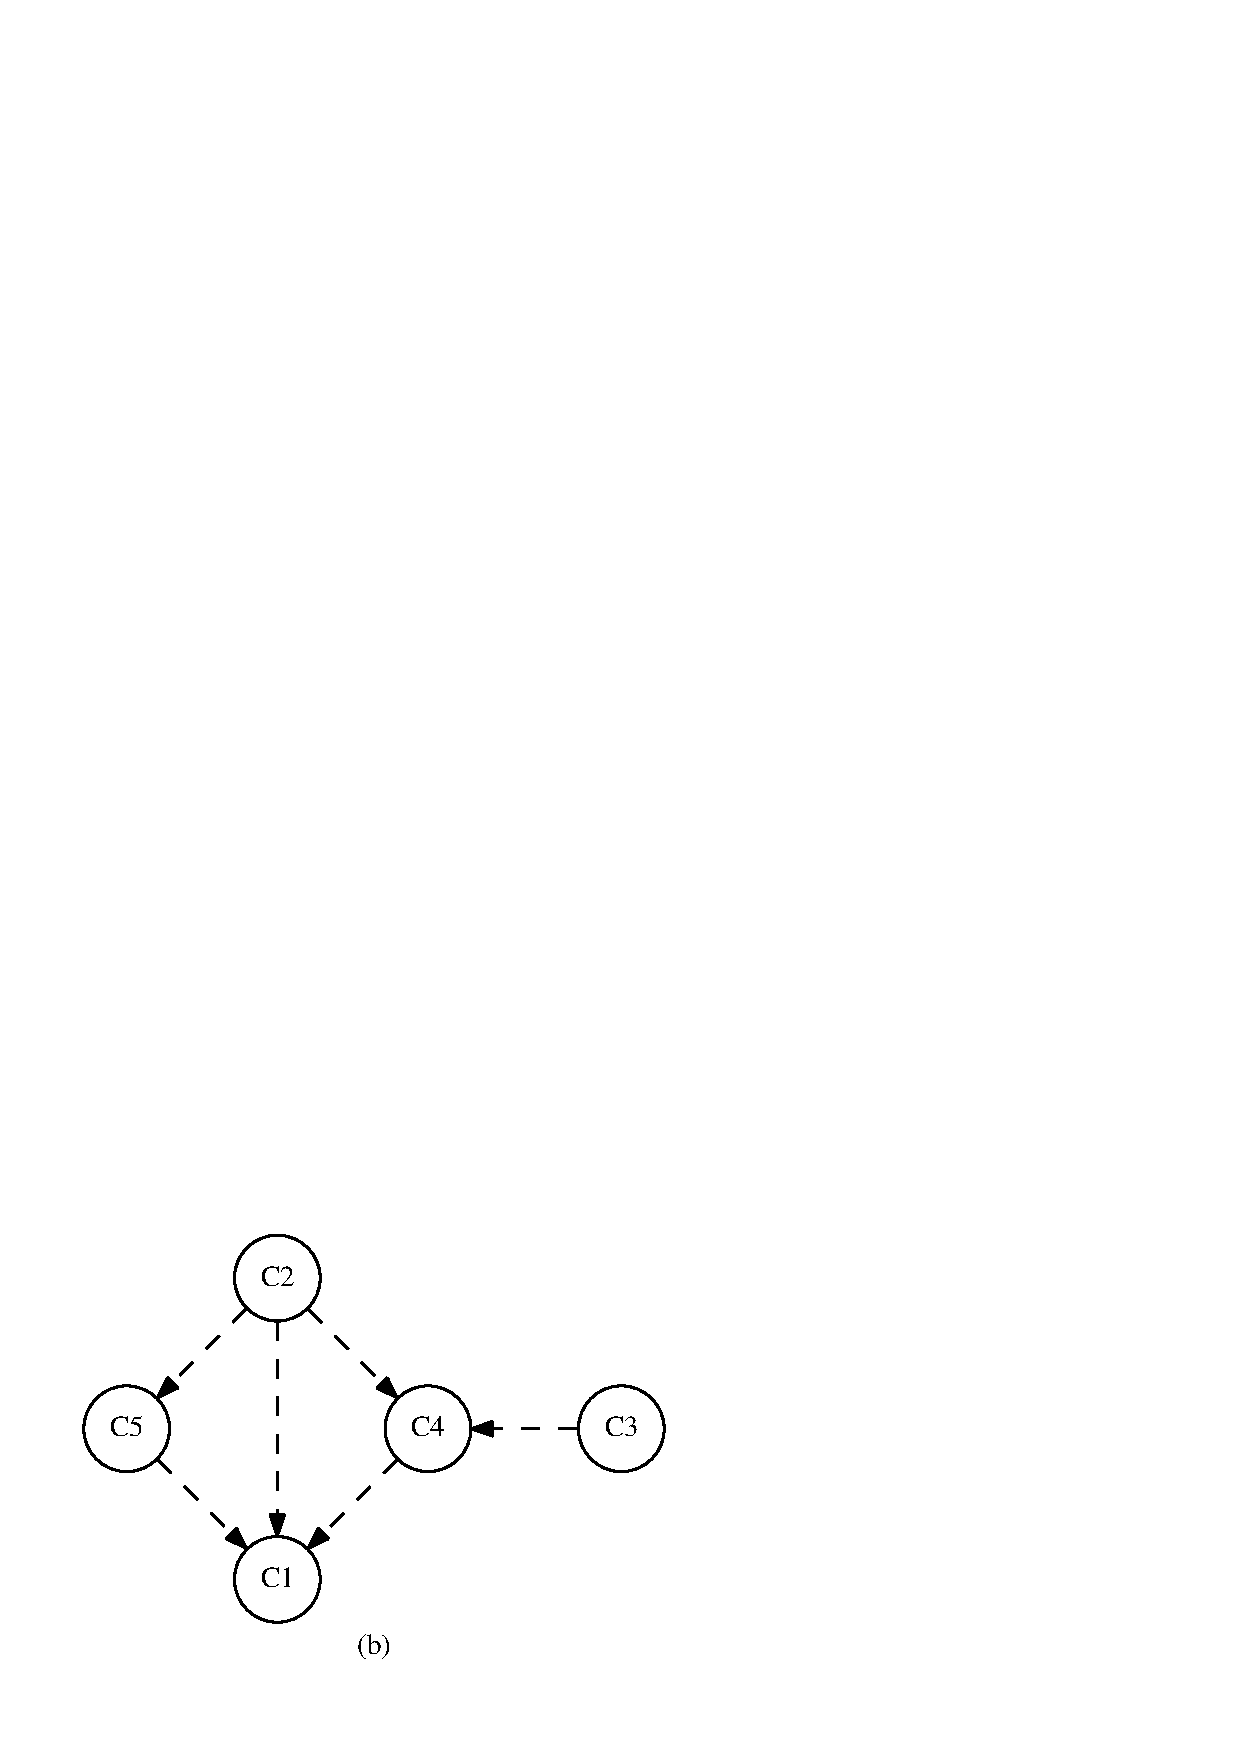
\includegraphics[width=0.57\columnwidth]{graphs/ccom.pdf}
%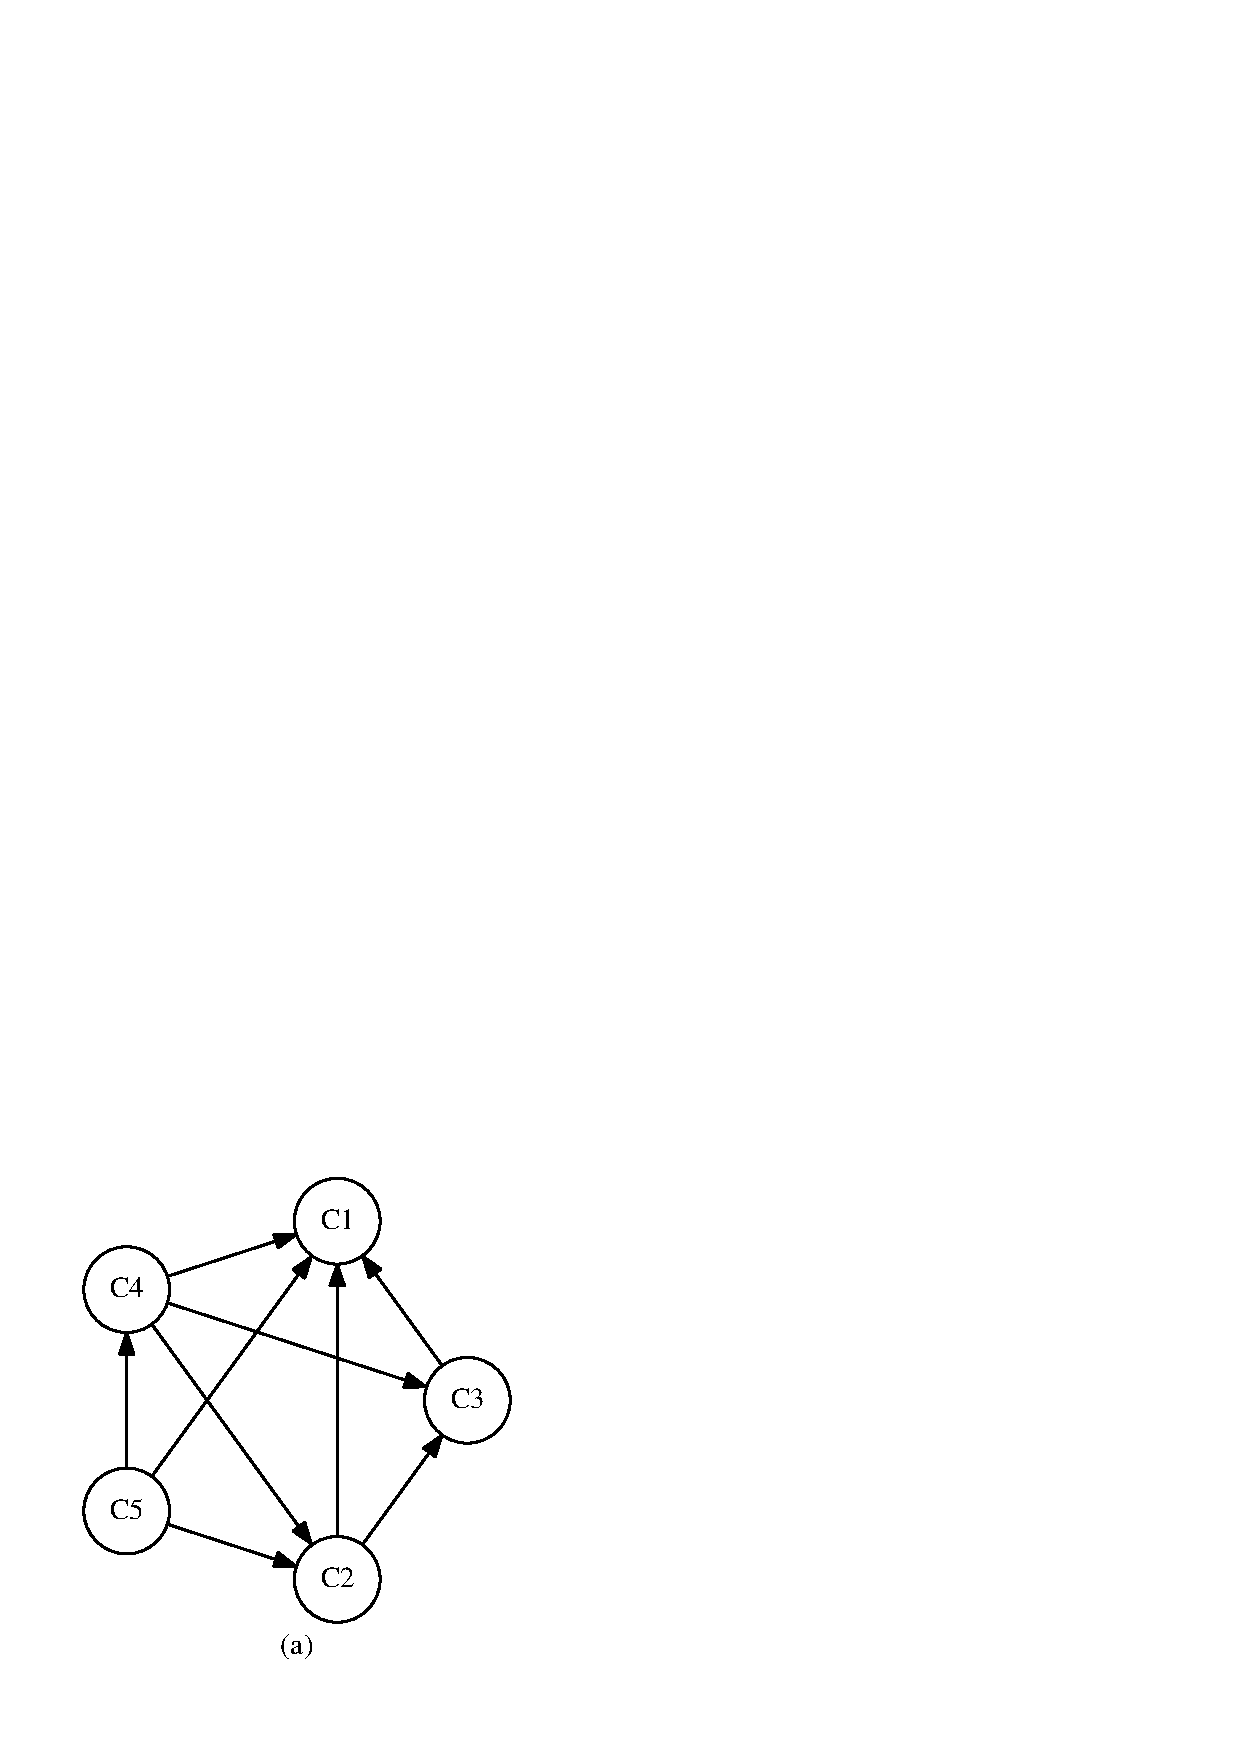
\includegraphics[width=0.40\columnwidth]{graphs/cart.pdf}
\includegraphics[width=0.57\columnwidth]{graphs/ccom.eps}
\includegraphics[width=0.40\columnwidth]{graphs/cart.eps}
\vspace{-12pt}
\caption{Trend graphs for the CCC equivalence graph: (a) represent the understandability analysis (RQ1) and (b) represent the artifact analysis (RQ2)}

\label{fig:graphsforanalysis}
\end{figure}


%\begin{table}
%\centering
%\caption{Topological Sorting, with the left-most position being highest \label{topologicalResults}}
%\begin{footnotesize}
%\begin{tabular}{| l | l | l | l | l | l |} \hline
%				& CCC			& DBB 		& LBW & SNG & LIT \\ \hline
%U 			& C1 C5 C4 C2 C3 	& D3 D1 D2 	& L3 L2		& S2 S1		& T1 T2 T4 T3 \\
%C		& C1 C3 C2 C4 C5 	& D2 D1 D3	&  L3 L2 L1 	& S2 S1 S3 	& T1 T3 T2 T4 \\
%\hline
%\end{tabular}
%\end{footnotesize}
%\end{table}

\begin{table}
\centering
\caption{Topological Sorting, with the left-most position being highest (non-smelly) and the right-most being most smelly \label{topologicalResults} \todo{make sure this matches new results}}
\vspace{-6pt}
\begin{tabular}{| l | l | l |}  \hline
& Understandability & Community  \\ \hline 
CCC & C1 C5 C4 C2 C3  &   C1 C3 C2 C4 C5  \\
DBB & D3 D1 D2  &   D2 D1 D3\\
 LBW & L3 L2	 &  L3 L2 L1 	\\
 SNG &  S2 S1 &  S2 S1 S3 \\
 LIT & T1 T2 T4 T3 & T1 T3 T2 T4 \\
\hline
\end{tabular}
\vspace{-6pt}
\vspace{-6pt}
\end{table}


%In the understandability graph, we represent a directed edge  $\overrightarrow{C2C1}$ when match(C1) $>$ match(C2) \emph{and} compose(C1) $>$ compose(C2). When there is a conflict between match and compose, as is the case with T1 and T3 where match(T1) is higher but compose(T3) is higher, an undirected edge $\overline{T1T3}$ is used. When one metric has a tie, as is the case with composition in E9, we use the other metric to determine  $\overrightarrow{C5C1}$. An example understandability graph for the CCC is shown in Figure~\ref{fig:graphsforanalysis}b. Nodes with few incoming edges are less understandable (or were not evaluated in our study), and nodes with more incoming edges were more understandable. 
%\footnote{When there are confounded representations, as is the case with E8, E4, and E5 which all use tranformations from the CCC and the LIT equivalence classes, we omit those from the understandability graph. This makes sense since all use a transformation between T1 and T4 strongly favoring T1. }

\subsubsection{Topological Sorting}
Once the graphs are built for each equivalence class and each set of metrics, we apply a modified version of Kahn's topological sorting algorithm to obtain a total ordering. 
%The first modification is to remove all undirected edges since Kahn's operates over a directed graph. 
%To begin, any disconnected nodes are added to the end of the topologically sorted list $L$. 
%In Kahn's algorithm, all nodes without incoming edges are added to a set $S$, which represents the order in which nodes are explored in the graph. For each $n$ node in $S$, all edges from $n$ are removed and $n$ is added to a list $L$. If there exists a node $m$ that has no incoming edges, it is added to $S$.  In the end, $L$ is a topologically sorted list.
%\begin{algorithm}
%  \caption{Modified Topological Sort}\label{topological}
%  \begin{algorithmic}[1]
%\State  $L \gets$ []
%\State $S \gets$ []
%\State Remove all undirected edges (creates a DAG) \label{removeundir}
%\State Add all disconnected nodes to $L$ and remove from graph. If there is more than one, mark the tie. \label{markTie1}
%\State Add all nodes with no incoming edges to $S$. If there is more than one, mark the tie. \label{addnoincomingtos}
%\While {$S$ is non-empty} \label{beginwhile}
%	\State remove a node $n$ from $S$ \label{setn}
%	\State add $n$ to $L$  \label{addntoL}
%	\For {node $m$ such that $e$ is an edge $\overrightarrow{nm}$}
%		\State remove $e$
%		\If{$m$ has no incoming edges}
%			\State add $m$ to $S$ \label{addToS}
%		\EndIf
%	\EndFor
%	\State If multiple nodes were added to $S$ in this iteration, mark the tie \label{markTie2}
%	\State remove $n$ from graph
%\EndWhile
%\State For all ties in $L$, use a tiebreaker.
%  \end{algorithmic}
%\end{algorithm}
One downside to Kahn's algorithm is that the total ordering is not unique and often multiple nodes with similar properties (e.g., no incoming edges) could be considered tied. Thus, we mark ties in order to identify when a tiebreaker is needed.
% to enforce a total ordering on the nodes (though admittedly, it is not always unique). 
%For example, on the understandability graph in Figure~\ref{fig:graphsforanalysis}, there is a tie between C3 and C2 since both have no incoming edges, so they are marked as a tie. Further, if C3 is added to $S$ first, when $n=C2$, both C5 and C4 are added to $S$, thus the tie between them is marked. In these cases, a tiebreaker is needed.
Breaking ties on the community standards graph involves choosing the representation that appears in a larger number of projects, as it is more widespread across the community. 
Breaking ties in the understandability graph uses the RQ1 results. Based on Table~\ref{table:testedEdgesTable}, we compute the average metrics for all instances of each representation. For example, C4 appears in E5, E12 and E13 with an overall average matching score of 0.81 and composition score of 24.3. C5 appears in E4 and E9 with an average matching of 0.87 and composition of 28.28. Thus, C5 is favored to C4 and appears higher in the sorting.

\subsection{Results}
The total orderings on nodes for each graph are shown in Table~\ref{topologicalResults}.  For example, given the graphs in Figure~\ref{fig:graphsforanalysis}a and Figure~\ref{fig:graphsforanalysis}b, the topological sorts are {\tt C1 C5 C4 C2 C3} and  {\tt C1 C3 C2 C4 C5}, respectively.



Considering both topological sorts, there is a clear winner in each equivalence class, with the exception of DBB.
%That is, the node sorted highest in the topological sorts for both the community standards and understandability analyses are 
This is C1 for CCC, L3 for LBW, S2 for SNG, and T1 for LIT.
Having a consistent and clear winner is evidence of a preference with respect to community standards and understandability, and thus provides guidance for potential refactorings.

%While the least-smelly representation is relatively clear, the smelliest representation varies.
%After the top rank, the second rank varies depending on the metric, however, h
This positive result, that the most popular representation in the corpus is also the most understandable, makes sense as people may be more likely to understand things that are familiar or well documented. However, while L3 is the winner for the LBW group, we note that L2 appears in slightly more patterns.
DBB is different  as the orderings are completely reversed depending on the analysis, so the community standards favor D2 and understandability favors D3. Further study is needed on this, as well as  LBW and SNG since not all nodes were considered in the understandability analysis. 
%


